\chapter{Diagrams modelisation}

In order to produce a visual schema from a SpinalHDL program, we need to parse
his AST and produce an intermediate model for the diagrams. The reason to use
an intermediate model is that we could then build multiple backend generator
for multiple output target. The complete pipeline of the generation is visible
in figure \ref{fig:generation-pipeline}.

\begin{figure}[H] % {{{ figure
    \centering
    \fbox{
        \digraph[scale=0.5]{GenerationPipeline}{
            node [shape=record];
            graph [rankdir=LR,
                   ranksep="1",
                   nodesep="1"];
            S [label="SpinalHDL"];
            I [label="Intermediate model"]
            S -> I;
            I -> JSON;
            I -> dot;
        }
    }
    \caption[KlugHDL generation pipeline]{This figure show the entire generation pipeline use by KlugHDL in order to generate different output. The intermediate model is use to produce the target code, for example dot or JSON file}
    \label{fig:generation-pipeline}
\end{figure} % }}}

We also need to introduce an crucial element to understand how the model is build : the hierarchy visualization.

\section{Hierarchy visualization}

The diagrams produces by KlugHDL are kind of special, they are hierarchical ones. That's means we need to find a way to show the hierarchy between the components of a SpinalHDL program. There is multiple way to do this :
\begin{itemize}
  \item Showing the elements using a hierarchical layout, like in family tree
  \item Showing the elements using a tree view, like in file explorer
  \item Showing the elements one by one (multiple diagrams)
\end{itemize}

\subsection{Hierarchical layout}
\label{sec:hierarchical-layout}

The hierarchical layout is the simplest way to achieve the visualization of the hierarchy. The figure \ref{fig:hierarchical-layout-simple} illustrate a simple hierarchical layout with some children and parent.

\begin{figure}[H]
  \centering
  \fbox{
  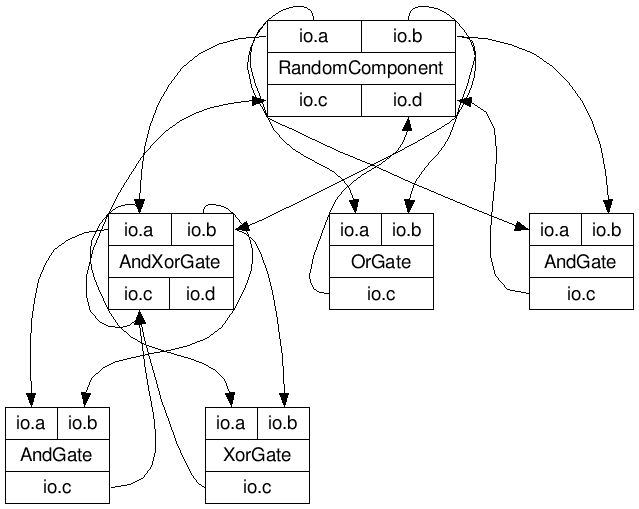
\includegraphics[width=0.7\textwidth]{img/HierarchicalLayoutSimple}
  }
  \caption[Simple hierarchical layout for diagram visualization]{The simplest
    hierarchical visualization, the parent are just representing using the height}
  \label{fig:hierarchical-layout-simple}
\end{figure}

The problem by using such a representation is clearly visible, sometimes the
ports of a component is an output type port as well as a input type port.
This can be seen at the port "io.c" from the \texttt{AndXorGate} component.

\subsection{Tree view}

The idea of the tree view is to represent the hierarchical relation like in file
explorer. The figure \ref{fig:tree-view} show the idea for a SpinalHDL
component.

\begin{figure}[H]
  \centering
  \fbox{
    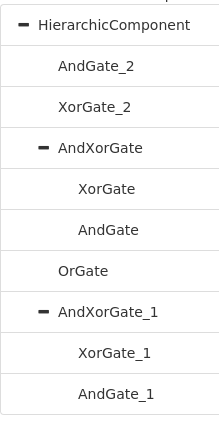
\includegraphics[width=0.2\textwidth]{img/tree-view}
  }
  \caption[SpinalHDL's Component visualization with tree view]{A tree view
    visualization of a SpinalHDL Component, each son are under his parent and
    eventually possesses it self some sub-Component}
  \label{fig:tree-view}
\end{figure}

The tree view visualization is very usefull to directly detect the relation
between some components. The big problem is that we can't see the connections
relationship.

\subsection{Multiple diagrams}

As seen with the hierarchical layout figure
\ref{fig:hierarchical-layout-simple}, the problem is that sometimes a port is an
output for somes components and, in the other way, an input for somes others
ones. If we look closely to the problems we could notice that a port receive
connections from his brothers and send connections to his childrens.

\begin{figure}[H]
  \centering
  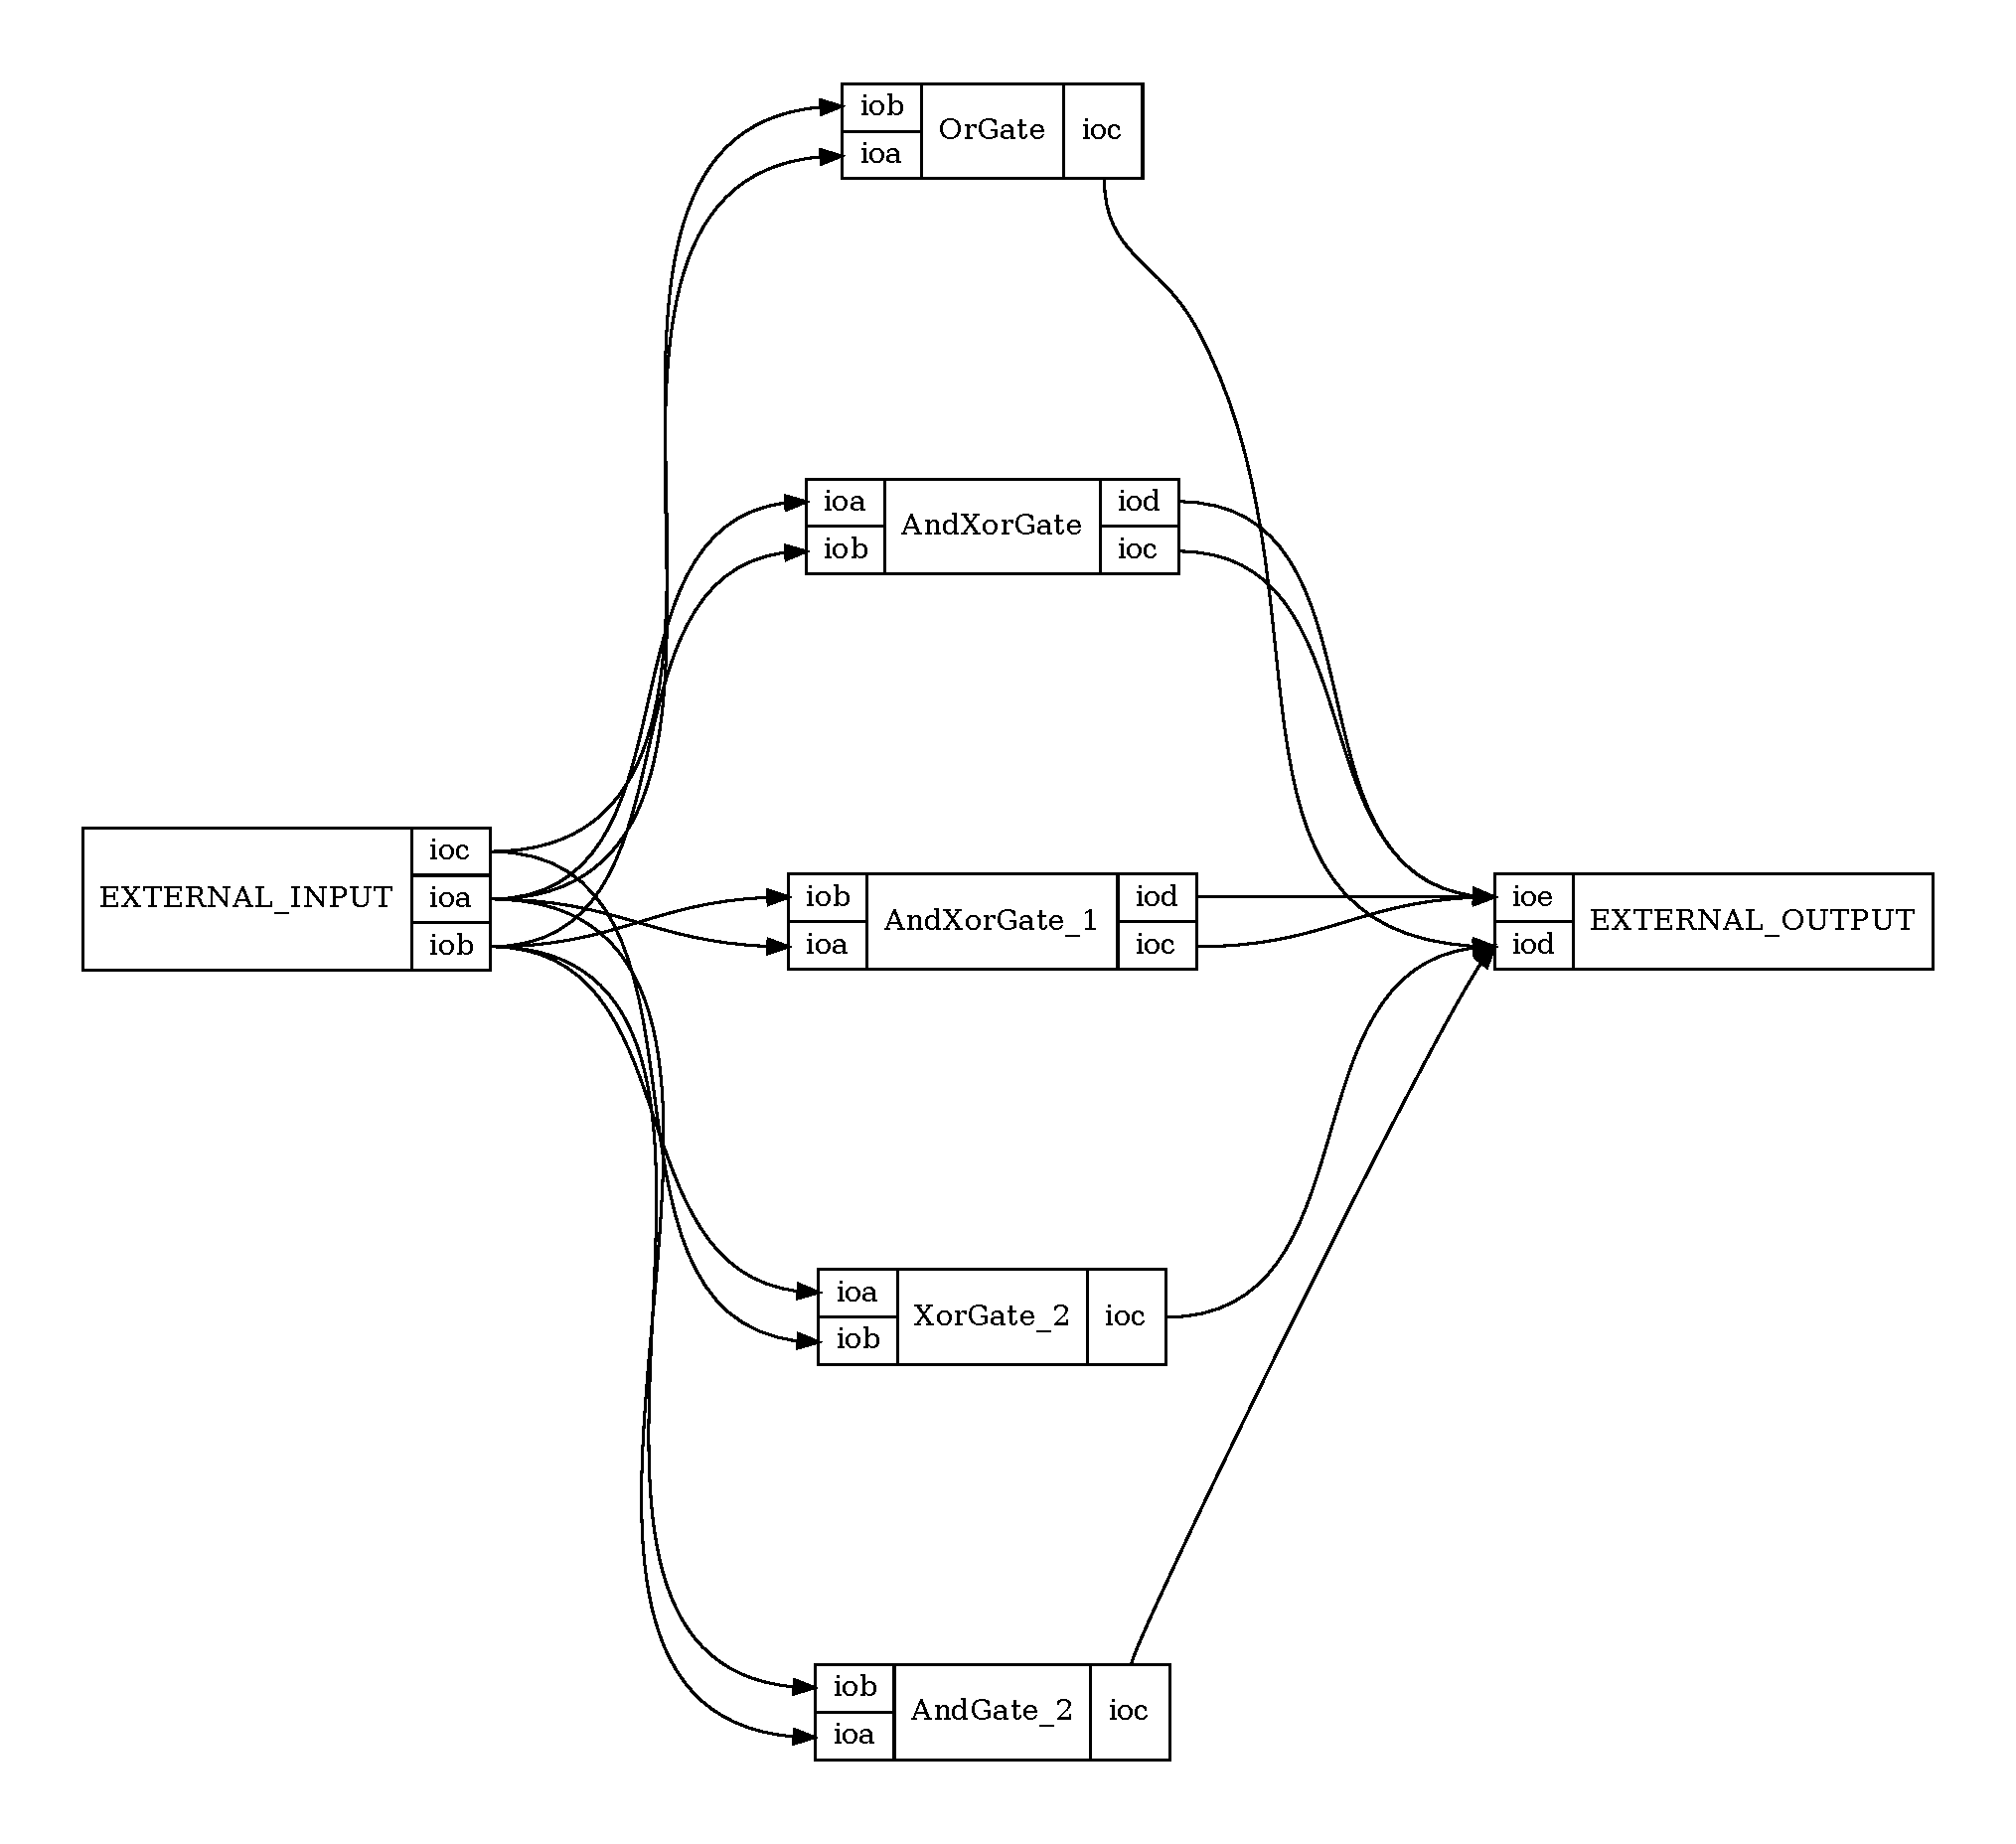
\includegraphics[width=0.6\textwidth]{img/HierarchicComponent.pdf}
  \caption[SpinalHDL Component inside]{Inside of a SpinalHDL components, the
    components possesses input and output has his own interface and communicates
  with his children}
  \label{fig:hierarchic-component}
\end{figure}

\begin{figure}[H]
  \centering
  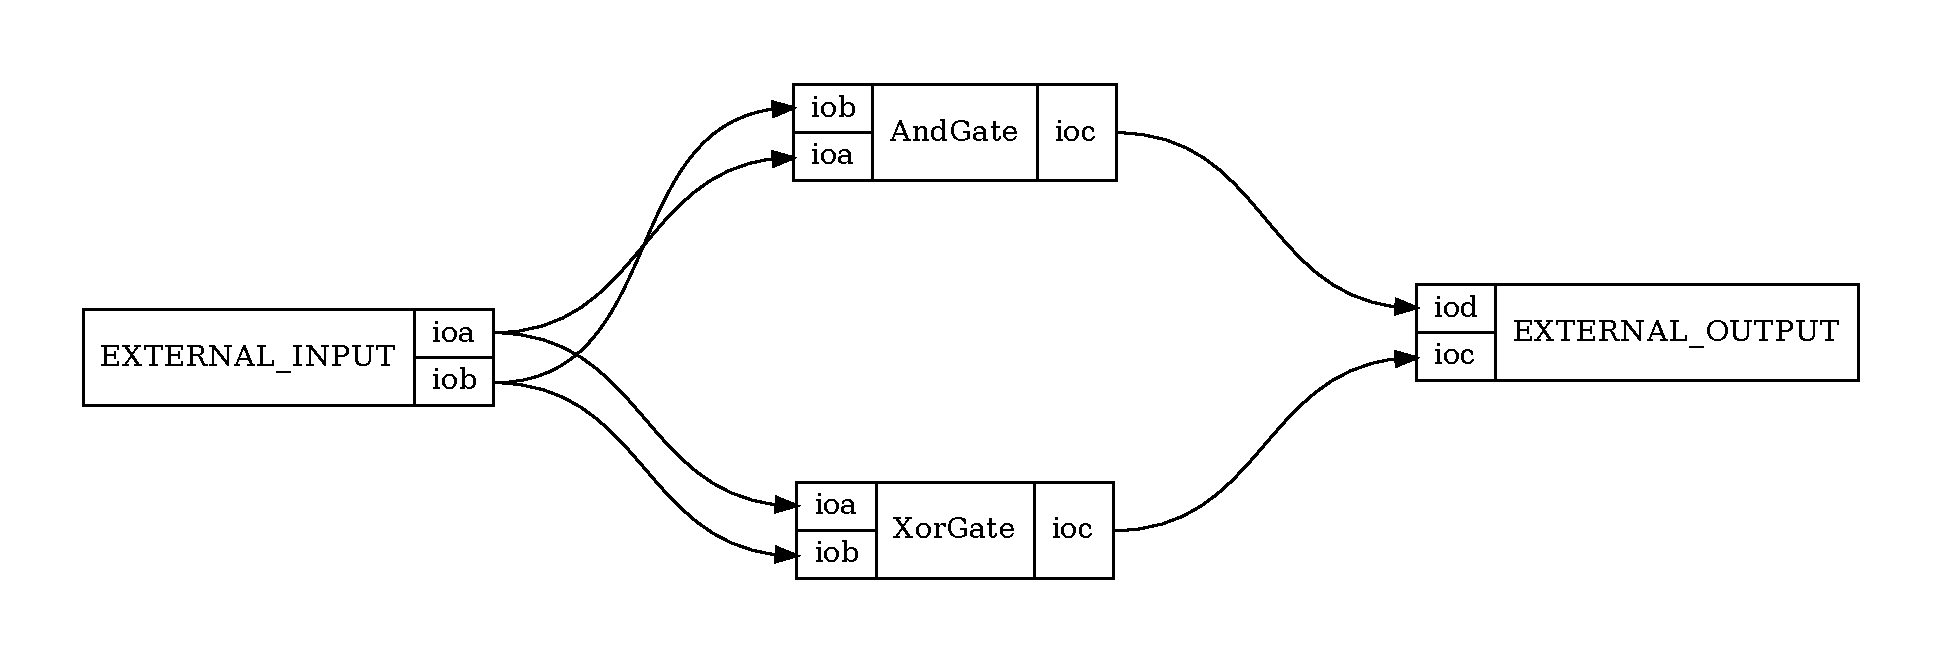
\includegraphics[width=0.6\textwidth]{img/AndXorGate.pdf}
  \caption[SpinalHDL Component inside an another]{Component which is the
    sub-component of the component from figure \ref{fig:hierarchic-component},
    the external inputs and outputs corresponding to the ones in the parent component}
  \label{fig:and-xor-gate}
\end{figure}

Using such a representation solve the problem discuss in
\ref{sec:hierarchical-layout} : if we represent all the components juste using
one diagram, sometimes the ports are inputs and sometimes they are outputs. With
multiple diagram this problem no more occurs.

The major disadvantages is that we need an interractive diagrams for exploring
the children of a components or multiple statics ones which is not practical.

\section{A visual example}

The diagram we want to produce, as explain in \ref{sec:graph-layout}, ownes the following property :
\begin{itemize}
  \item Oriented
  \item Cyclic
  \item Connection between port on nodes and not between nodes
\end{itemize}

\section{Model representation}

The model representation is builded using the oriented-object paradigm, the figure \ref{fig:model-class-diagram} show the class diagram of the models.

\begin{figure}[H]
  \centering
  \fbox{
  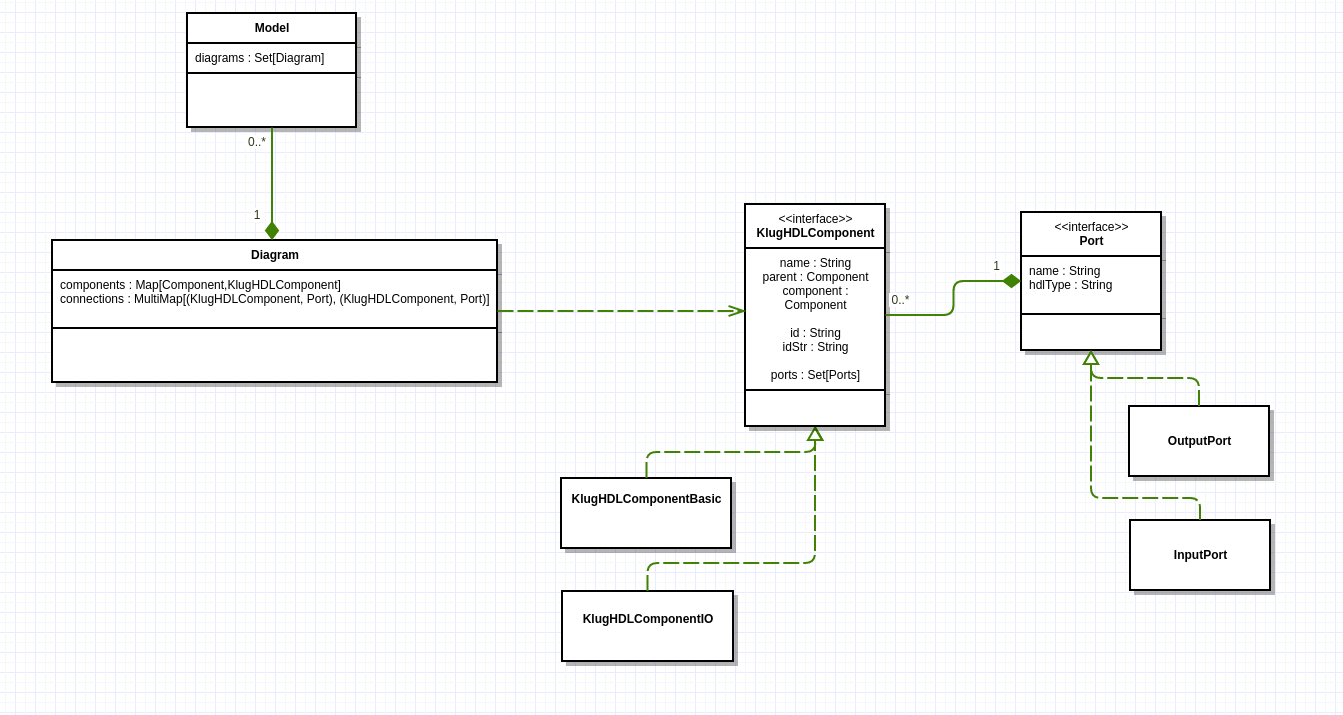
\includegraphics[width=0.99\textwidth]{img/class-diagram-intermeditate-model}
  }
  \caption[Class diagram of the intermediate model]{The complete class diagram of the intermediate model representation}
  \label{fig:model-class-diagram}
\end{figure}

\section{Conclusion}

The major advantages of such an intermediate representation is the capability to evolve the program in order to produce additionnal output. For now there is just a \textbf{dot} and \textbf{JSON} backend. It's also provide a way to check the correctness of the diagram after the parsing on the AST : connections with non-existing port for example.
